\begin{titlepage}
\begin{center}

% Upper part of the page. The '~' is needed because \\
% only works if a paragraph has started.

\textsc{\LARGE INSA Rennes}\\[1.5cm]

\textsc{\Large Jeu Small World}\\[0.5cm]

% Title
\HRule \\[0.4cm]
{ \huge \bfseries Rapport de conception \\[0.4cm] }

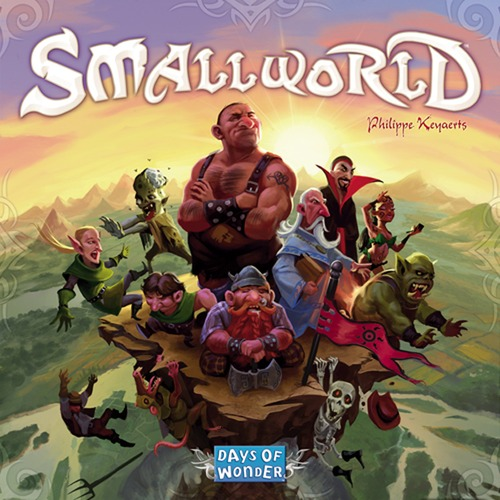
\includegraphics[width=0.8\textwidth]{./images/smallworld.jpg}~\\[1cm]


\HRule \\[1.5cm]

% Author and supervisor
\begin{minipage}{0.4\textwidth}
\begin{flushleft} \large
\emph{Auteurs :}\\
Loïck \textsc{Bonniot}\\
Quentin \textsc{Dufour}\\
\end{flushleft}
\end{minipage}
\begin{minipage}{0.4\textwidth}
\begin{flushright} \large
\emph{Enseignants :} \\
Eric \textsc{Anquetil}\\
Arnaud \textsc{Blouin}\\
Maud \textsc{Marchal}\\
Pascal \textsc{Fresnay}\\
\end{flushright}
\end{minipage}

\vfill


\end{center}
\end{titlepage}
